\documentclass{extarticle}

\usepackage{graphicx}
\usepackage{enumerate}
\usepackage{amsthm}
\usepackage{amsmath}
\usepackage[margin=1.0in]{geometry}

\begin{document}

\begin{titlepage}
\title{Design Document for Kairos Constraint-Based Scheduling Software System}
\author{Tyler Chapman, Nate Crandall, Vinh Dang, Vince Oveson, Tony Tuttle}
% INSERT TEAM LOGO
\maketitle
\thispagestyle{empty}
\end{titlepage}

\tableofcontents

\newpage

\section{Executive Summary} % ONE PAGE

\subsection{Overview}
% DESCRIBE THE FINAL GOAL OF THE PROJECT
%   - what the project will do
The final goal of the project is to provide a highly customizable, open-source, web-based scheduling tool available
to solve a wide range of scheduling problems.  Our software system will be accessible through a public
website where users may build, modify, and maintain their solutions.  The system will be capable of solving various
types of scheduling problems for various types of user needs.

%   - what need it will address
Scheduling problems are ubiquitous.  Individuals, teams, organizations, and larger entities such as companies all
must solve scheduling problems of various levels of complexity.  Our tool aims to address the needs of such a wide
base of potential users.

\subsection{Features and Components}
% LIST KEY FEATURES AND COMPONENTS
%   - schedule solver
%   - web-based (open to all users)
%   - customizable
%   - well-written API
%   - thoughtful visualization component
At its core, Kairos will be a web-based schedule solver; it will accept parameters from the user, specifying the
details of their particular scheduling problem.  The tool will analyze the input and algorithmically determine a
schedule that will meet all of the supplied parameters.  If meeting all of the constraints is not possible, it will
prioritize based on weights and determine what compromises to make in the schedule.

Since the tool will be web-based, it will be open to any and all potential users.  This will further encourage a
wide breadth of users.

We intend to make the tool extremely customizable by creating a very general schedule solver core.
We want users to have access to the powerful core components while maintaining sufficient flexibility to fit the
solution to their specific needs.

Part of this customizability will come from working hard to make the API as clear and thorough as possible.  A
great piece of software may lose potential users if it is not clear to users how best to leverage the software.  We
intend to encourage a large user base by putting a lot of emphasis on creating a strong API.

Likewise, a great piece of software that lacks intuitiveness or a pleasing user experience will alienate users.
We will put a great deal of thought and planning into determining how best to use visualization tools to represent
our data.  Since scheduling is a complex problem that produces data that will need to be viewed from several angles,
this is a difficult problem in itself.  By making visualization a priority we hope to attract users as opposed to
driving them away.

\subsection{Justification}
% EXPLAIN WHY THE PROJECT IS INTERESTING AND WORTHWHILE
%   - why a completed project will be beneficial
Making this tool available to the public will potentially save individuals a great deal of time, provide
organizations better scheduling solutions than they currently have, and save a great deal
of money for businesses and other organizations.  At the very least, it is our hope that we will make life a little
easier for as many users as possible.

\section{Background}

\subsection{Overview} % ONE TO THREE PAGES
%   - why our project is needed
The task of creating optimal schedules is a problem that event planners, groups, teams, and other organizations of
all sizes encounter on a regular basis.  The schedules used by these groups are often created manually.  For all
but the simplest schedules, this task is extremely complicated and time consuming.  As the complexity increases,
the difficulty of creating acceptable schedules, much less optimal ones, increases exponentially.

%   - what problems it solves
Moving as much of the work of scheduling from a manual process to one that is solved by a computer is the
inspiration for Kairos.  Kairos has the potential to save a great deal of time for users.  Kairos will provide a
better solution for those who need to schedule any but the simplest of events.

%   - who will use it
Since scheduling is a ubiquitous problem, Kairos will be usable to large number of users.  By implementing a
well-documented API we intend to attract those who seek a solution that they can tweak to fit their specific needs.

A specific use case that we have identified is the School of Computing at the University of Utah.  We are working
with staff in the department to provide a solution to their problem of scheduling classes each semester.

\subsubsection{Similar Ideas}
% list, describe other software systems that do what ours will do
We have identified two software systems that address the scheduling problem in some manner similar to that which
we are aiming at.  These systems are Aurora Intelligent Planning and Scheduling System (Aurora) and Microsoft
Project (MS Project).  To be sure, there are other software systems out there, but these are adequate to represent
the current state of this space.

\subsubsection{How Kairos is Different}
% explain why our idea is different and/or better
Based on their literature, Aurora addresses the needs that we are attempting to address more than adequately.
However, they are focused on supplying solutions to very large organizations with correspondingly very large
scheduling problems.  We would like to address the needs of the smaller users for which the Aurora software would
be overkill.

While MS Project does include scheduling tools in the software package, the larger goal of MS Project is to provide
project management software.  Thus, their software is attempting to address a problem with a wider scope than we
are focused on.  Based on reading the literature on their software, it is not clear that the scheduling tools
provided in MS Project are constraint-based scheduling tools.

Both Aurora and MS Project cost money.  Our software will be free.  Neither Aurora or MS Project are web-based, but
require installation on any machine that will use the software.  There is certainly room for our tool in this
space.

\subsection{Required Technology}
% list, describe software technologies that you will:
%   - need to implement
%   - need to utilize
Our project can be broken down into three main components:  a core web service, specific modules that connect to
it, and an API that handles communication between the two.  We will discuss the technologies we plan to utilize in
developing each of these three components.

\subsubsection{Core Web Service}
This is where the logic for the schedule solver will live.  This web service will be centered around the transfer
of data through requests and responses.  Our web service will use API keys to restrict access.  In order to
authenticate users, we will store these keys in a MySQL database.  This will make our web service more secure.

\subsubsection{SoC Module}
We will create a module for the School of Computing that connects to our web service.  This module will be a web
application that allows the user to specify the events (classes) to be scheduled, the resources to be used
(professors, rooms, etc.), and the constraints for both classes and resources.  When the web service sends back a
suggested schedule, the user will be provided with different options for viewing the data.  We also plan to provide
some web scraping tools in order to facilitate the collection of data relevant to scheduling classes.

This module with have a PHP backend, along with a MySQL database.  The front end will be built using HTML,
JavaScript, and CSS.  We will utilize jQuery (specifcally ajax) to make asynchronous requests to the web
service without interrupting the user experience.

\subsubsection{API}
Our API will use JSON to represent the data being shuttled back and forth between the web service and the modules
which connect to it.  We plan to provide detailed documentation that will help other developers leverage our
service in their own applications.  To make this documentation readily available and accessible, we will create a
website where we will publish the API documentation, and also advertise our service.  This site will also be where
developers can request an API key.

\subsection{Assets and Engines}
% assets and engines
%   - how much will be built from scratch
%   - what resources, assets (and from where) will be leveraged
The websites we create -- both the API documentation site and the School of Computing module -- will be built using
the Laravel Artisan PHP framework.  This will provide structure to our web sites, as well as allow us to keep our
code organized and concise.  Laravel also includes a command line interface which will provide us with shortcuts
for common tasks, thus allowing us to focus our efforts on more important development tasks.

\subsection{Software/Hardware Requirements for Users}
% what hardware, software we will need to successfully installed in order to use our software
Since Kairos will be a web application with all of the intensive computation taking place on our network, the only
system requirements for users will be a machine running a modern browser with a reasonably fast internet connection.

\newpage

\appendix
\section{Use Cases}

\subsection{Entering Data Manually to Create a New Schedule}
The user will manually enter the data required for the system to generate a proposed schedule.  The steps for this
use case are:

\begin{enumerate}
\item User navigates to Manual Data Entry page
\item System prompts user to enter classes
\item User enters classes and selects `Next'
\item System prompts user to enter rooms
\item User enters rooms and selects `Next'
\item System prompts user to enter professors
\item User enters professors and selects `Next'
\item System prompts user to enter constraints on room availabilities
\item User enters constraints on room availabilities and selects `Next'
\item System prompts user to enter constraints on professor availabilities
\item User enters constraints on professor availabilities and selects `Create Schedule'
\item System calculates and returns a proposed schedule to user
\end{enumerate}

See the related Figure~\ref{fig:upload_csv} on page~\pageref{fig:upload_csv}

\subsection{Uploading a CSV File to Create a New Schedule}
The user will generate a proposed schedule by uploading the required data via a .csv file.  The steps for this use
case are:

\begin{enumerate}
\item User prepares spreadsheet for upload
\item User navigates to CSV Import page
\item System prompts user to enter path to file for upload
\item User enters path and selects `Upload'
\item \label{upload.parse} System attempts to parse scheduling data from file
  \begin{enumerate}
  \item If the parse fails
    \begin{enumerate}
    \item Failure is minimal
      \begin{enumerate}
        \item System prompts user to adjust data
        \item User adjusts data
        \item Return to [\ref{upload.parse}] above
      \end{enumerate}
    \item Failure is large
      \begin{enumerate}
        \item System informs user of error
        \item System returns user to Dashboard page
      \end{enumerate}
    \end{enumerate}
  \end{enumerate}
\item System calculates and returns a proposed schedule to user
\end{enumerate}

\subsection{Exporting Schedule as a CSV File}
The user will download a local copy of a proposed or modified schedule as a .csv file.  The steps for this use
case are:

\begin{enumerate}
\item User navigates to one of the View pages on an existing schedule
\item User clicks Export to CSV option
\item Browser prompts user to accept download
\item Browser begins download of CSV file
\end{enumerate}

% ADD THE RELATED UI SKETCH

\subsection{Modifying a Proposed Schedule} \label{usecase.modify}
The user will make modifications to an existing schedule that they created.  They will change the parameters
of a given class in order to change some feature of the class.  The steps for this use case are:

\begin{enumerate}
\item User navigates to one of the View pages on an existing schedule
\item User right clicks on an instance of a class and selects `Modify This Class'
\item System displays the resources and constraints for that class and prompts user to modify as needed
\item User modifies the resources/constraints and selects `Modify Schedule'
\item System calculates and returns a proposed schedule with the modifications to user
\end{enumerate}

% ADD THE RELATED UI SKETCH

\subsection{Importing a New Schedule}

The user will create a new schedule by uploading a .csv file. This is useful for new users wanting to work on existing schedule created from outside our software. The csv file is similar to that used in importing data use case, but it contains the schedule itself instead of the scheduling data. The steps for this use case are:

\begin{enumerate}
\item User prepares csv file for upload. The file should contain Class, Time, Room, and Professor as columns as a least.
\item User clicks on `Import schedule' button from the dashboard
\item \label{usecase.import_schedule.upload} System prompts user to enter path to file for upload
\item User enters path and selects `Upload'
\item System reads schedule information from file, and returns the schedule to user for review
	\begin{enumerate}
	\item In case of failure, system shows an error message and returns to step \ref{usecase.import_schedule.upload}
	\end{enumerate}
\item User saves the schedule to system.
\end{enumerate}

See related Figure~\ref{fig:upload_csv} on page~\pageref{fig:upload_csv}.

\subsection{Marking for Schedule Revision}

Users added to a schedule should be able to mark things for future revision. Only the schedule's owner is able to make direct changes (refer to use case \ref{usecase.modify}). The steps for this use case are:

\begin{enumerate}
\item User opens the schedule from the Dashboard page
\item \label{usecase.marking.select} On one of the Schedule View pages, user right clicks on an instance of a class and selects `Mark this class for revision'
\item System prompts user to enter reason for the marking
\item User enters the reason and click Save
\item (Optional) System returns to the schedule view page. User can make further marking for revision from there (return to step \ref{usecase.marking.select})
\end{enumerate}

\subsection{Checking Notification}

User should be able to check changes/markings for revision coming from schedules they have access to. There are two user roles in our system: The schedule's owner and the normal user (users added to a schedule by the owner). The roles are heavily tied to each schedule, and hence, a user can be both a schedule's owner and a normal user at the same time. In this use case, the term user will be used in general when the user role doesn't matter, or when it has been specified in that context. The steps for this use case are:

\begin{enumerate}
\item User will see a notification badge, together with the total number of notifications, on the top side bar
\item After clicking on the badge, user will be redirected to a new page with all the notifications information (the person, schedule, and class it comes from)
	\begin{enumerate}
	\item For schedule's owner, notifications will see markings for revision coming from other users
	\item For normal user, notifications will be changes, or `marking for revision' status made by the schedule's owner
	\end{enumerate}
\item If notification is a marking for revision, or a change made by the schedule's owner, clicking on the notification will bring the user to the schedule view page with the affected class being focused
\item If the notification is a marking for revision (for schedule's owner only):
	\begin{enumerate}
	\item User right clicks on the notification and select either `Approve' or `Reject'
	\item If choosing `Reject', system prompts user to enter comment
	\item If choosing `Reject', user enters comment and clicks `Save', or doesn't enter anything and clicks `Skip'
	\end{enumerate}
\item If the notification is a `marking for revision' status (for normal user only), clicking on the notification will show the status and the detailed comment.
\end{enumerate}

\subsection{Comparing Two Schedules}
The user will select two existing schedules for comparison.  The system will display the discrepancies between the
two schedules.  The steps for this use case are:

\begin{enumerate}
\item User creates and saves at least two schedules
\item User navigates to the dashboard page
\item User selects `Compare Two Schedules'
\item System prompts user to select two schedules for comparison
\item User selects two schedules and selects `Compare'
\item System calculates the differences between the schedules and displays them simultaneously, highlighting the
differences
\end{enumerate}

%ADD THE RELATED UI SKETCH
  
\subsection{Administrative Tasks}
The schedule administrator will be able to load, delete, rename, update users who can view the schedule, and accept/reject 
changes made by other users of the schedule.
\begin{enumerate}
\item User creates and saves a schedule
\item User logs in to the system
\item User goes to the dashboard
\item User selects the schedule(s) that need to be updated.
\item The user can then select their administrative task(i.e. load, delete) on the right sidebar
\end{enumerate}

%ADD THE RELATED UI SKETCH

\subsection{API use}
The third party developer will request a key and create their own implementation of a constraint based scheduling 
system using our api.

\begin{enumerate}
\item The developer will request an api key
\item The developer will read the api website to learn how to use our api
\item The developer will send the request he needs
\item The system will return json data that the developer can parse and use
\end{enumerate}

\appendix
\section{UI Sketches}

\begin{figure}[h!]
\label{fig:upload_csv}
\centering
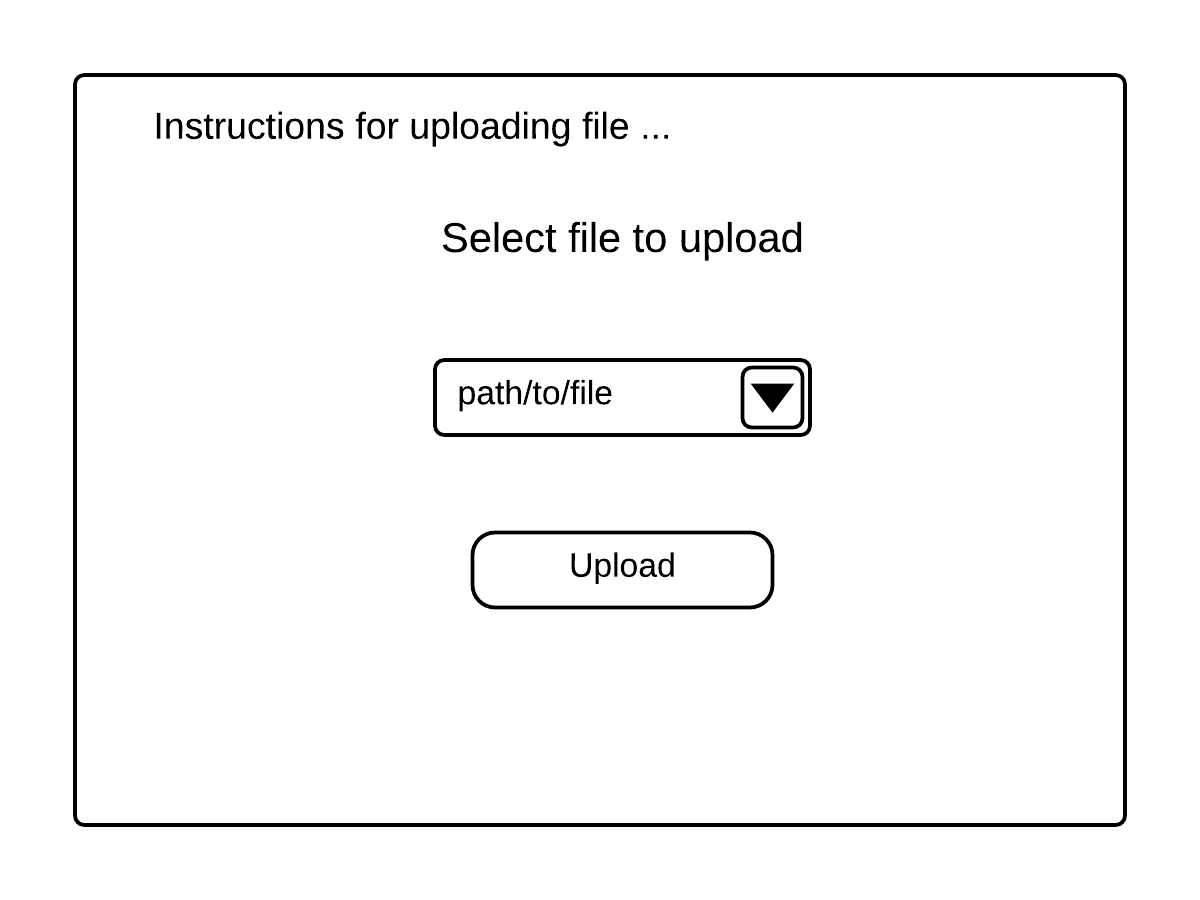
\includegraphics[width=1.0\textwidth]{upload_page_wireframe}
\caption{Wireframe of UI for user to upload a CSV file}
\end{figure}

\end{document}
